\documentclass{standalone}
\usepackage{tikz}
\usepackage{pgfplots}
\usepgfplotslibrary{statistics}
\pgfplotsset{compat=1.16}
\begin{document}
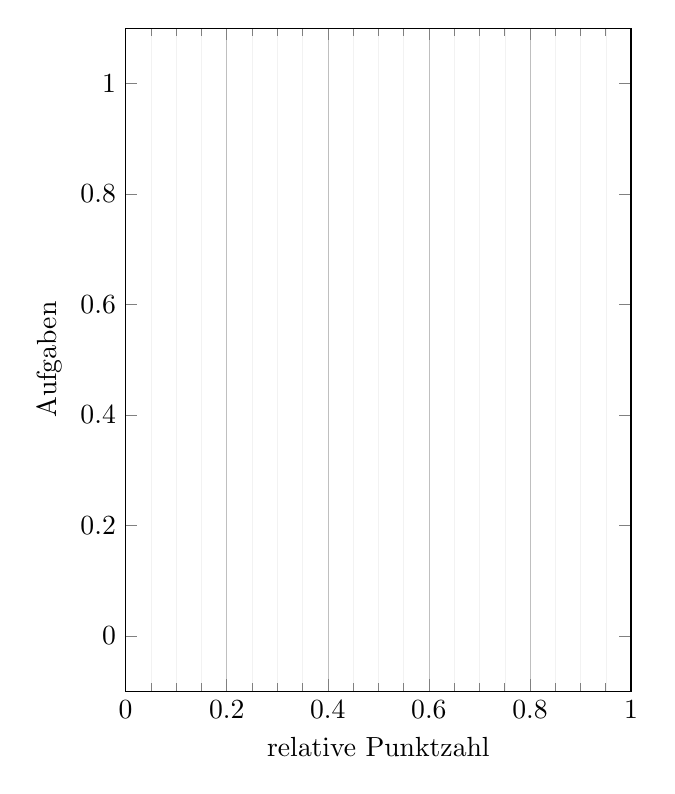
\begin{tikzpicture}
	\begin{axis}[
		xmin=-0.125, xmax=1.375,
		xlabel={relative Punktzahl},
		ylabel={Aufgaben},
		xtick={0, 0.25, ..., 1.25},
		% yticklabels
		yminorticks=false,
		ymajorgrids=false,
		yminorgrids=false,
		xmajorgrids=true,
		xminorgrids=true,
		grid style={line width=.1pt, draw=gray!10},
		major grid style={line width=.2pt,draw=gray!50},
		width=8cm, height=10cm,
		minor x tick num = 3,
		minor y tick num = 0,
		]
		% neue Plots
		%\addplot+[
		%boxplot prepared={
			%lower whisker = <Min>,
			%lower quartile = <UQ>,
			%median = <MD>,
			%average = <MW>,
			%upper whisker = <Max>,
			%upper quartile = <OQ>
	\end{axis}
\end{tikzpicture}
\end{document}
